\documentclass{beamer}

\usetheme[
    block=fill,
    background=light,
    titleformat=smallcaps,
    numbering=none
]{metropolis}

\usepackage{tabularx}
\usepackage{wasysym}
\usepackage{amsmath}
\usepackage{amssymb}
\usepackage{mathtools}
\usepackage{proof}
\usepackage{stmaryrd}
\usepackage{pifont}

\usepackage{tikz}
\usetikzlibrary{calc}
\usetikzlibrary{matrix}

% Decorated Arrow
\newlength{\arrow}
\settowidth{\arrow}{\scriptsize$10$}
\newcommand*{\myrightarrow}[1]{\xrightarrow{\mathmakebox[\arrow]{\text{\scriptsize #1}}}}

\title{From Raw Text to Linear $\mathbf{\lambda}$-Terms}
\author{Konstantinos Kogkalidis}
\institute{Compositionality in formal and distributional models of natural language}
\date{July 2019}

\begin{document}

\maketitle

\begin{frame}{Overview}
    \alert{Big Question}\\
    Where do $\lambda$-terms come from anyway?

    \pause
    \alert{A syntactic framework for Semantic Compositionality}\\
    \begin{itemize}
        \item[1] Type Logic
        \item[2] Type Lexicon
        \item[3] Type Assignment (Supertagging)
        \item[4] Parsing \& Surface Form
    \end{itemize}
\end{frame}

\section{Logic}
\begin{frame}{Lambek Types, Lexical Ambiguity \& Wide Coverage}
\begin{tabularx}{1\textwidth}{@{}lcX@{}}
    \textbf{Phrase} & \textbf{Structure} & \textbf{Verbal Type} \\
    eenden eten$_1$ vis {\footnotesize\textit{ducks eat fish}} & SVO & $(\textsc{np}\backslash\textsc{s})/\textsc{np}$ \\
    eten$_2$ eenden vis? {\footnotesize\textit{do ducks eat fish?}} & VSO & (\textsc{s}/\textsc{np})/\textsc{np} \\
    eenden die vis eten$_{3,4}$ {\footnotesize\textit{ducks that eat fish}} & SOV & $\textsc{np}\backslash(\textsc{np}\backslash\textsc{s})$ \\
    eenden die vis eten$_{3,4}$ {\footnotesize\textit{ducks that fish eat}} & OSV & $\textsc{np}\backslash(\textsc{np}\backslash\textsc{s})$ \\
\end{tabularx}\\
\begin{center}
    \dots
\end{center}

\pause
\begin{align*}
\mathcal{L} := \text{eten}_1 &: (\textsc{np}\backslash\textsc{s})/\textsc{np}, \\
			\text{eten}_2 &: (\textsc{s}/\textsc{np})/\textsc{np} \\
			\text{eten}_{3,4} &: \textsc{np}\backslash (\textsc{np}\backslash \textsc{s}), \\
			\dots 
\end{align*}

\centering 
\frownie 
\end{frame}

\begin{frame}{Abstract Syntax with MILL}
    \alert{Inductive Type Scheme} \\
    \begin{align*}
        \mathcal{T}_A &:= A \ | \ T_1 \to T_2
    \end{align*}
    \alert{Logical Rules \& Computational Terms}
    \begin{align*}
    \begin{minipage}{0.5\textwidth}
		\[
	        \infer{\Gamma, \Delta \vdash s\langle t \rangle: B}{
	            \Gamma \vdash s: A \rightarrow B
	            &
	            \Delta \vdash t: A
	        }
	    \]
	    \end{minipage}    \begin{minipage}{0.5\textwidth}
	    \[
	        \infer{\Gamma \vdash \lambda x.u : A \rightarrow B}{
	            \Gamma, x: A \vdash u: B
	        }
	    \]
    	\end{minipage}
    \end{align*}
\end{frame}

\begin{frame}{Lexical vs. Structural Ambiguity}
    \alert{Smaller Lexicon}
    \begin{align*}
    \mathcal{L}' := \text{eten}_{1,2,3,4} &: \textsc{np} \to \textsc{np} \to \textsc{s} 
    \end{align*}

\pause
    \alert{More Proofs}
    \footnotesize 
    \vfill
    \[
    \infer[\rightarrow E]{\text{eenden}, \text{eten}, \text{vis} \vdash \textsc{s}}{
    	\infer[\rightarrow E]{\text{eten}, \text{vis} \vdash \textsc{np} \to \textsc{s}}{
    		\infer[\rightarrow Ax.]{\text{eten} \vdash \textsc{np} \to \textsc{np} \to \textsc{s}}{}
    		&
    		\infer[\rightarrow Ax.]{\text{vis} \to \textsc{np}}{}
    		}
    	&
    	\infer[Ax.]{\text{eenden} \vdash \texttt{eenden}: \textsc{np}}{}			
    }
    \]	
    \center \texttt{(eten vis) eenden} {\large\color{blue}\checkmark}
    \vfill
    \[
    \infer[\rightarrow E]{\text{eenden}, \text{eten}, \text{vis} \vdash \textsc{s}}{
    \infer[\rightarrow E]{\text{eten}, \text{eenden} \vdash \textsc{np} \to \textsc{s}}{
    	\infer[\rightarrow Ax.]{\text{eten} \vdash \textsc{np} \to \textsc{np} \to \textsc{s}}{}
    	&
    	\infer[\rightarrow Ax.]{\text{enden} \to \textsc{np}}{}
    	}
    &
    \infer[Ax.]{\text{vis} \vdash \textsc{np}}{}			
    }
    \]
    \center \texttt{(eten eenden) vis} {\large\color{red}\ding{55}}
\end{frame}

\begin{frame}{Dependency Decorations}
Replace $\to$ with dependency-decorated variants:
\begin{itemize}
	\item[] \{$\myrightarrow{su}$, $\myrightarrow{obj}$, $\myrightarrow{predc}$, $\myrightarrow{mod}$, \dots \}
	\item[] eten : $\textsc{np} \myrightarrow{obj} \textsc{np} \myrightarrow{su} \textsc{s}$
\end{itemize}
\pause
Lexical Preferences + Decorations $\implies$ \alert{reduced ambiguity} \\ 
\vfill
\pause
\alert{Formally}\\
Unary modality $\diamondsuit^d$ for $d$ $\in$ \{su, obj, predc, mod, \dots\}\\
    \begin{minipage}{0.4\textwidth}
\begin{align*}
        \infer{\langle \Gamma \rangle^d \vdash \diamondsuit^d A}{\Gamma \vdash A}\tag{$\diamondsuit^d I$}
\end{align*}
    \end{minipage}\begin{minipage}{0.6\textwidth}
\begin{align*}
        \infer{\Gamma [\Delta] \vdash B}{
        \Delta \vdash \diamondsuit^d A
        &
        \Gamma[\langle A \rangle^d] \vdash B
        }\tag{$\diamondsuit^d E$}
\end{align*}
    \end{minipage}
\end{frame}

\section{Lexicon}

\begin{frame}{Grammar Extraction}
    \alert{Goal}\\
    From syntactically-annotated corpora to type grammars
    \vfill 
    
    \pause 
    \begin{tabularx}{0.9\textwidth}{@{}c@{}c@{}c@{}}
        \textbf{ Lassy-Small} & \ $\to$ \  & \textbf{Type Grammar} \\
        \hline 
         $\sim$65\,000 sentences & \ $\to$ \  & Type Sequences \\ 
         $\sim$30 POS Tags \& Phrasal Categories & $\to$ & Atomic Types \\
         $\sim$30 Dependency Labels & $\to$ & Modal Decorations \\
         $\sim$1 mil words & $\to$ & Type Lexicon $\mathcal{L}$ \\
    \end{tabularx}
\end{frame}

{
\setbeamercolor{background canvas}{bg=gray!00}
\begin{frame}{Grammar Extraction: Example}
\begin{figure}
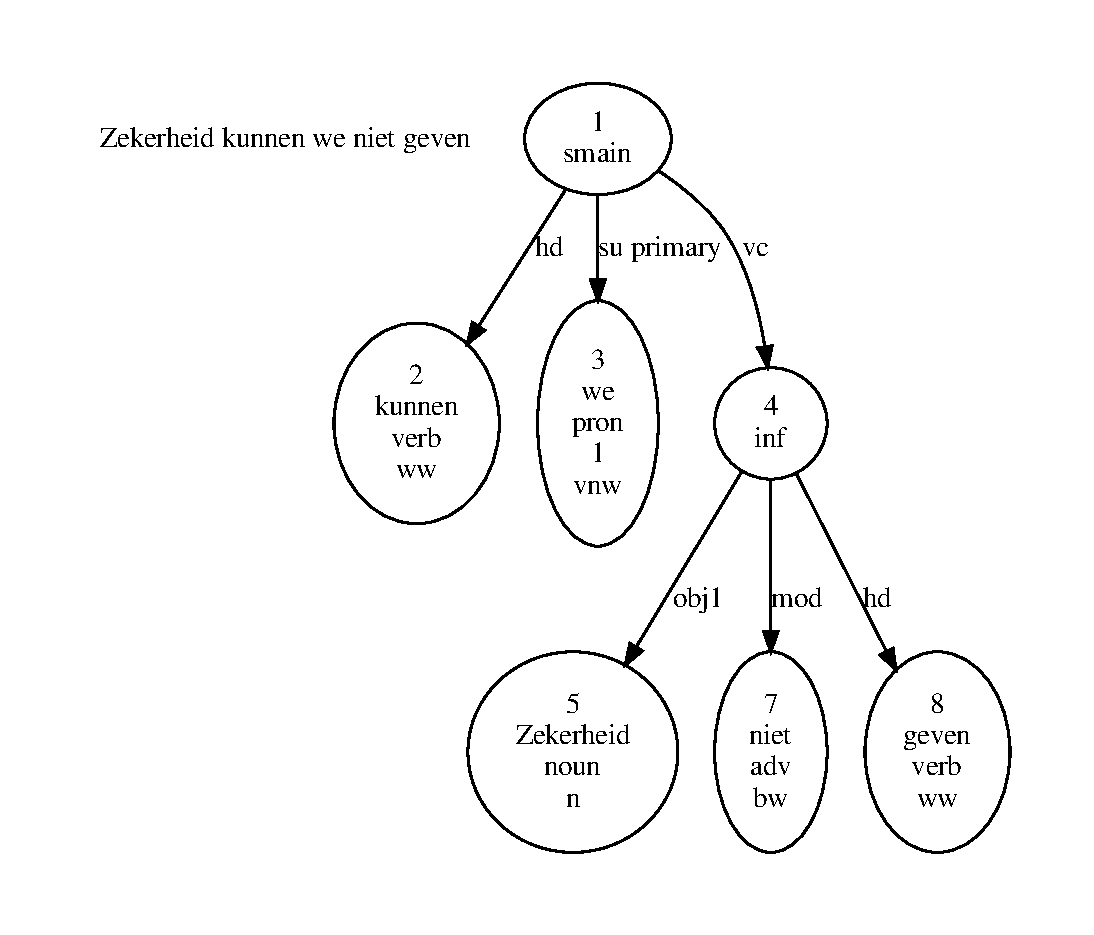
\includegraphics[scale=0.5]{zekerheid.pdf}
\end{figure}
\end{frame}
}

{
\setbeamercolor{background canvas}{bg=gray!00}
\begin{frame}{Extraction: Example}
\begin{figure}
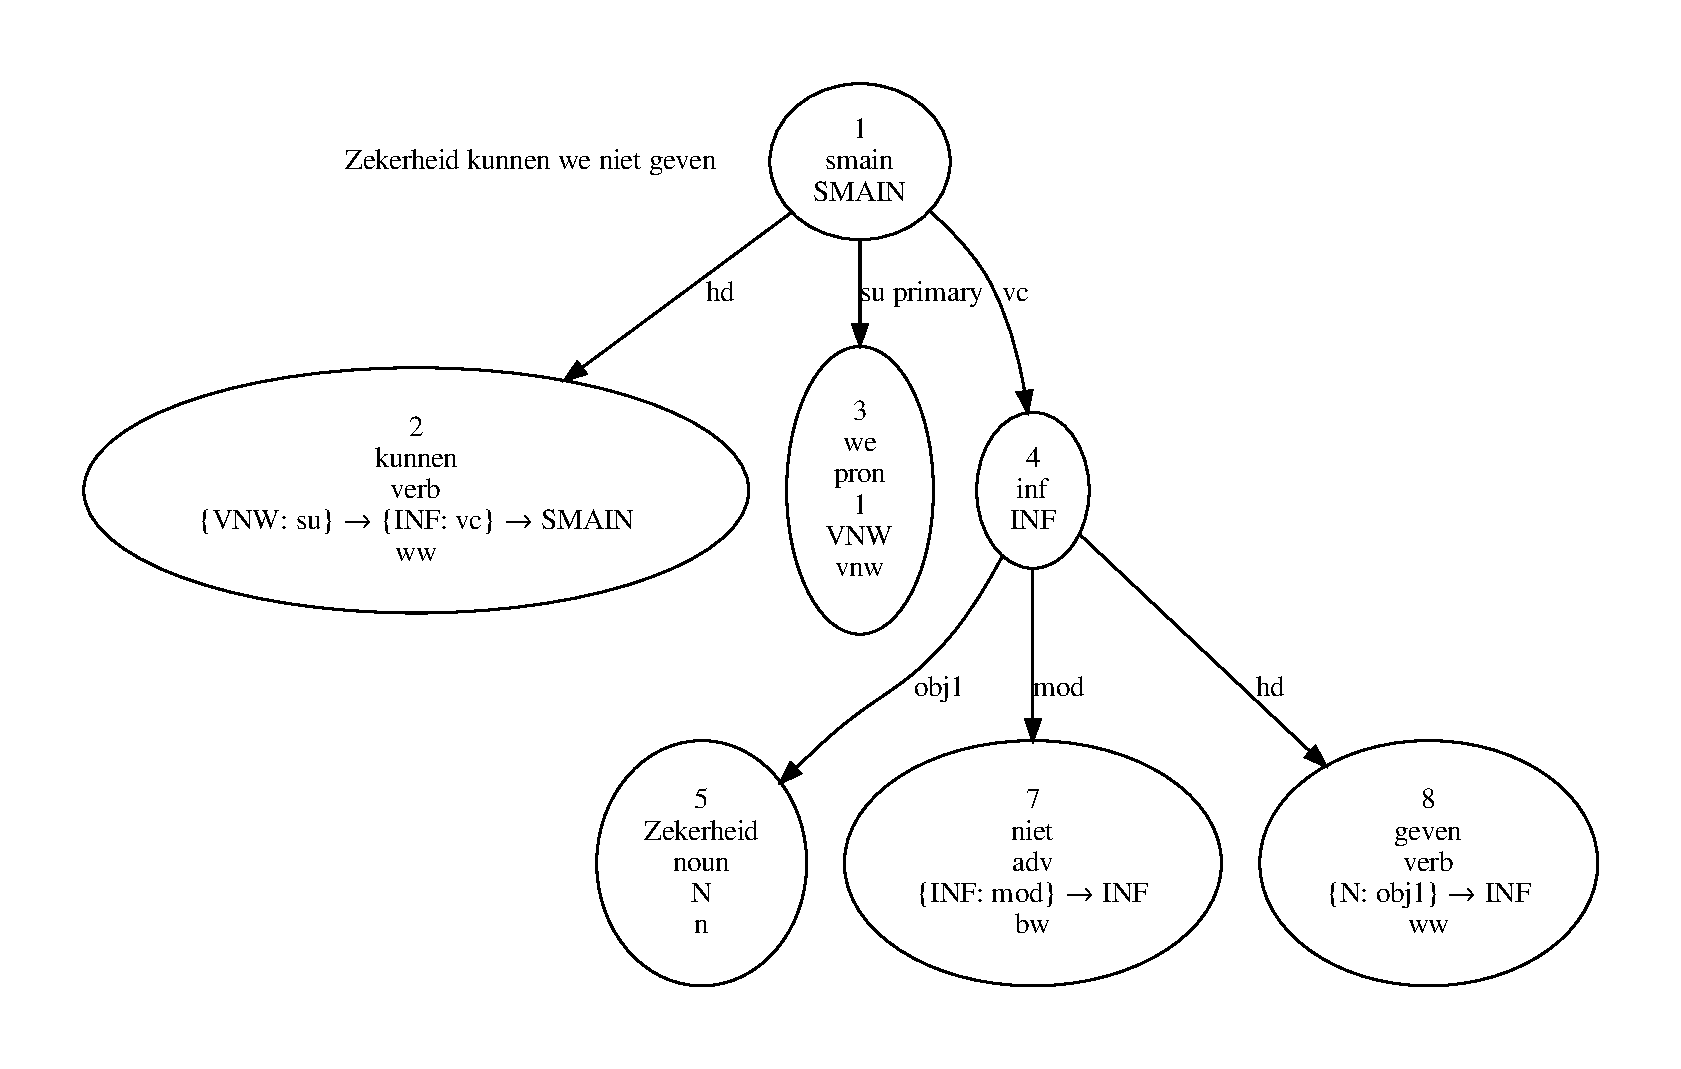
\includegraphics[scale=0.38]{zekerheid2.pdf}
\end{figure}
\end{frame}
}

{
\setbeamercolor{background canvas}{bg=gray!00}
\begin{frame}{Grammar Extraction: Lexicon}
\alert{Size} 
\begin{itemize}
    \item[] 70\,000 unique tokens 
    \item[] 6\,000 unique types (!)
\end{itemize}

\centering
\begin{figure}
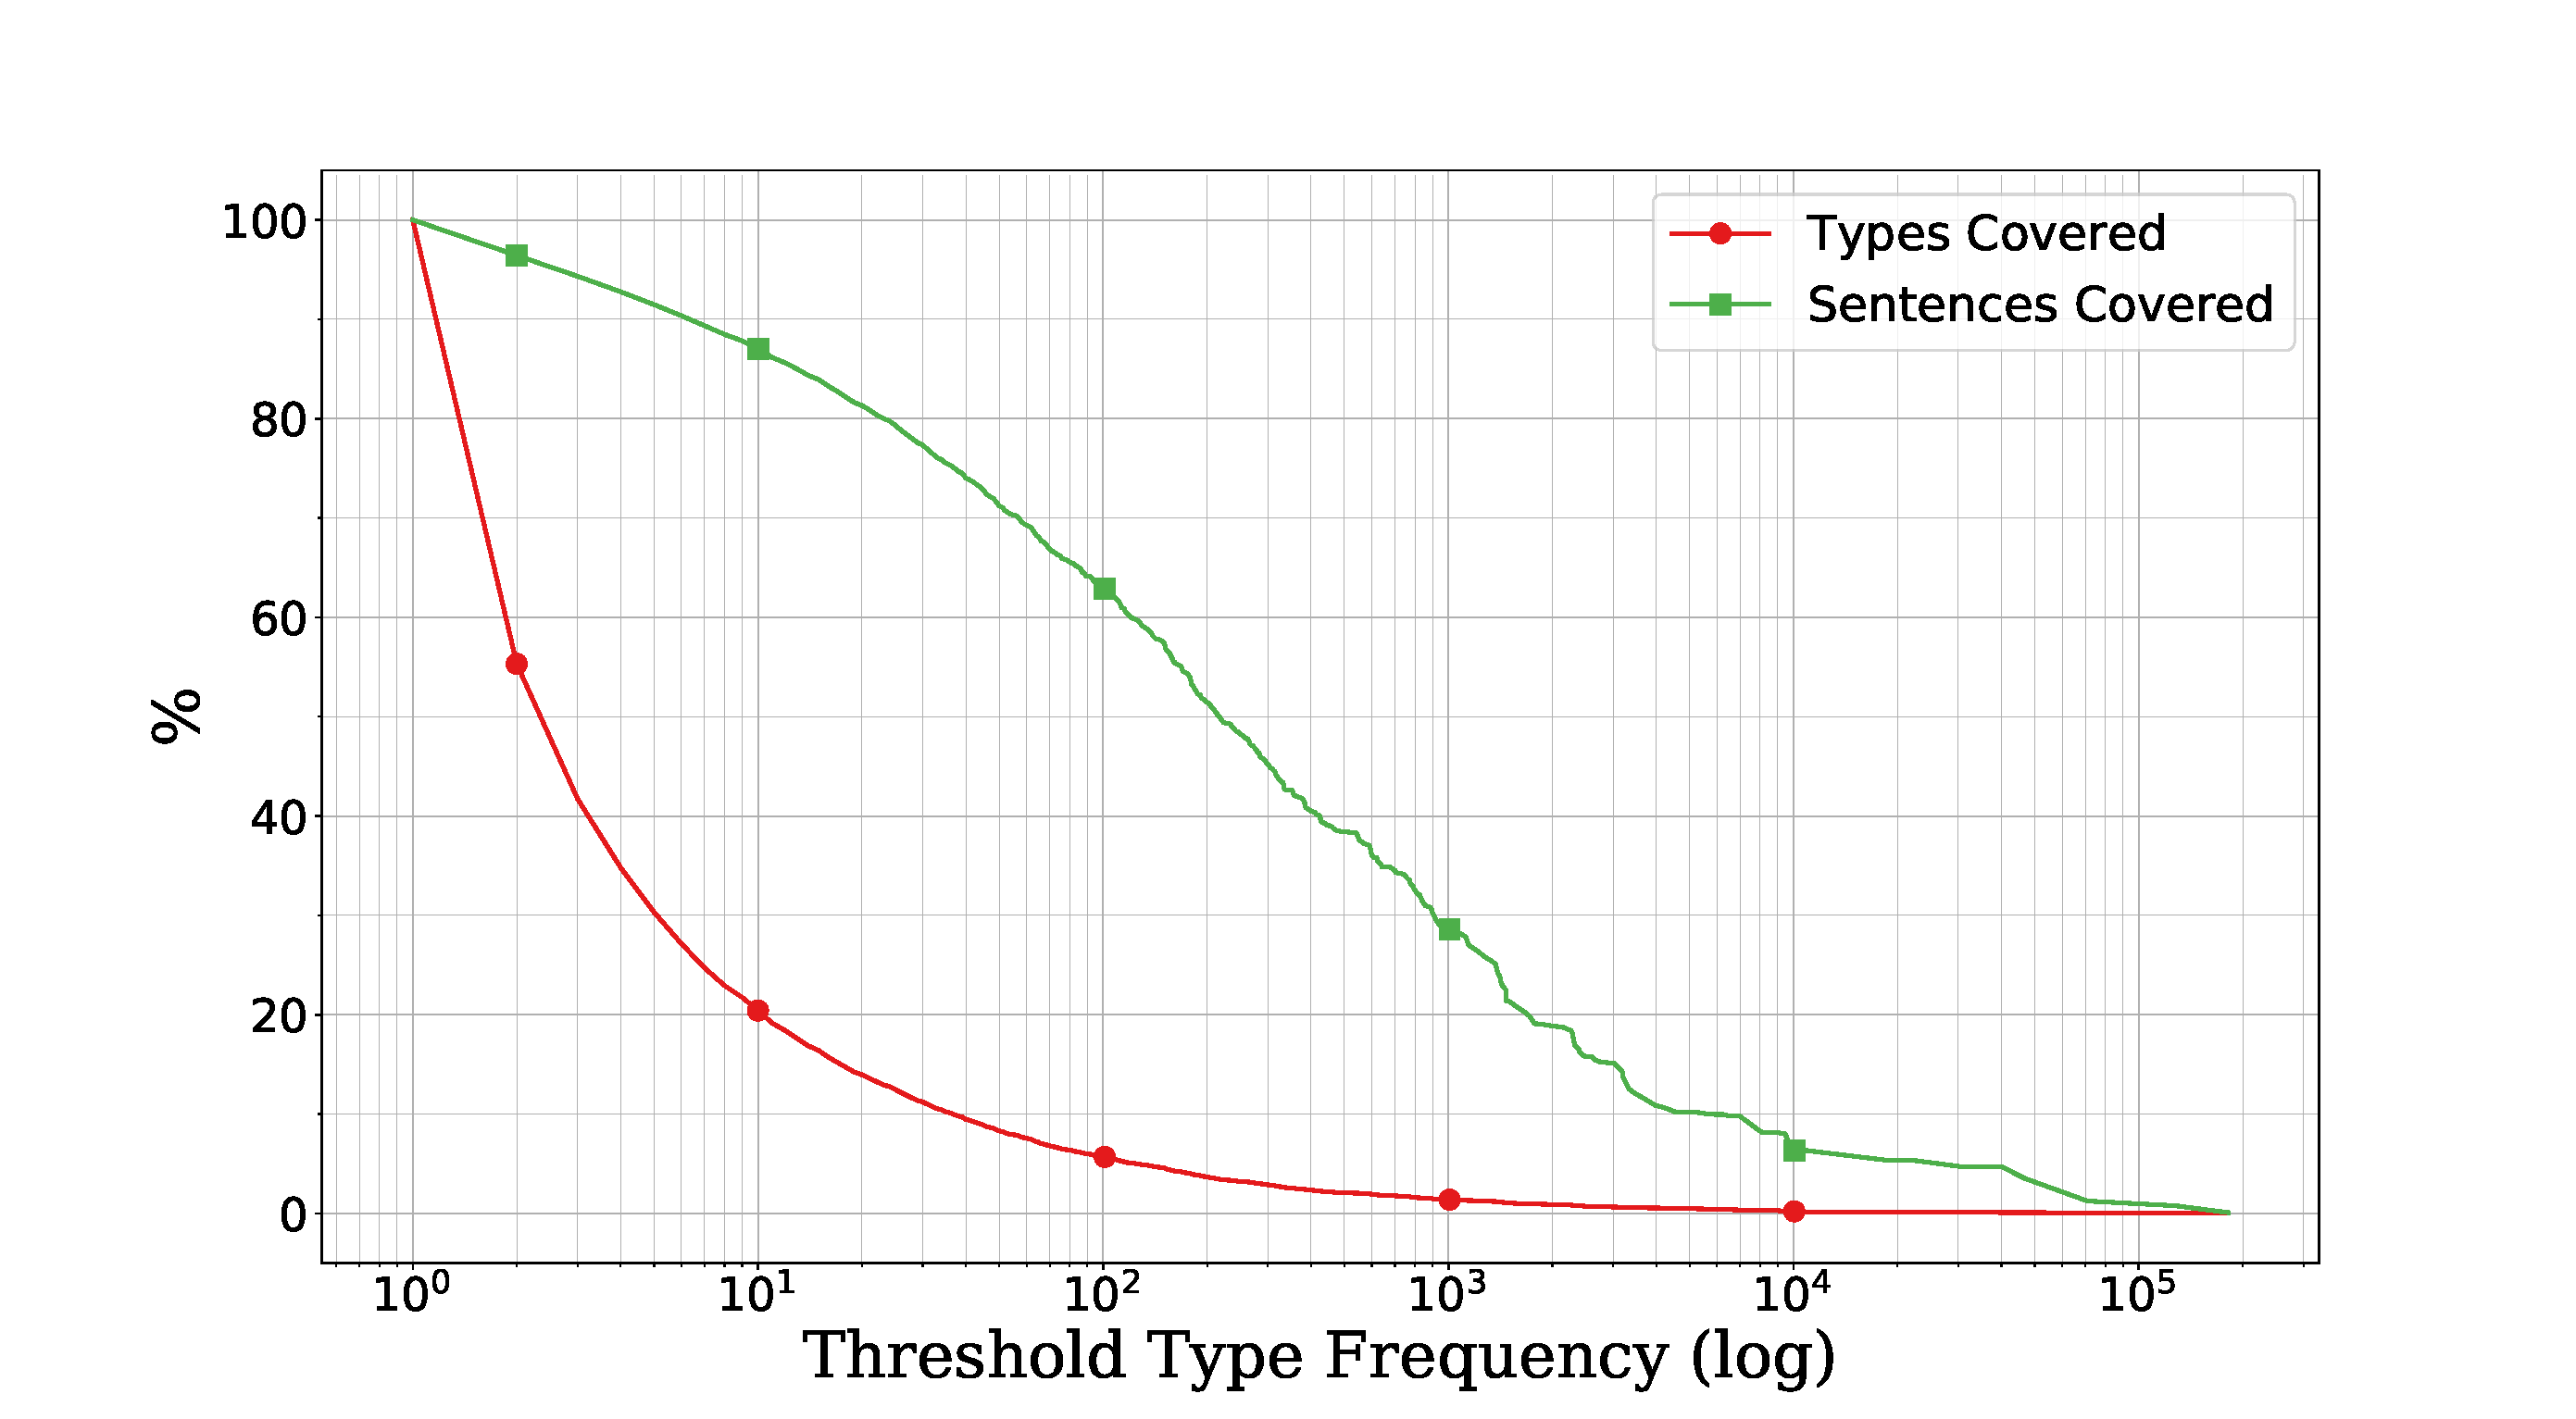
\includegraphics[scale=0.22]{sparsity.pdf}
\end{figure}
\end{frame}
}


\section{Supertagging}
\begin{frame}{Supertagging: Standard Approach}
\alert{Sequence Classification}\\
\quad Given input data sequence (word vectors) \\
\quad predict a class for each sequence item (types)
\vfill

\pause
\begin{figure}
\centering
\begin{tikzpicture}
	
	\node[rectangle, inner sep=0pt, minimum width=120pt, minimum height=20pt] (ducks) at (-2, -1.5) {eenden};
	\node[rectangle, inner sep=0pt, minimum width=120pt, minimum height=20pt] (eat) at (0, -1.5) {eten};
	\node[rectangle, inner sep=0pt, minimum width=120pt, minimum height=20pt] (fish) at (2, -1.5) {vis};
	
	\node[draw=white, rectangle, minimum width=160pt, minimum height=20pt, ultra thick, fill=black] (bb) at (0, 0) {\color{white}{Black Rectangle}};
	
	\pause
	\node[rectangle, inner sep=0pt, minimum width=120pt, minimum height=20pt] (ducks) at (-2, -1.5) {eenden};
	\node[rectangle, inner sep=0pt, minimum width=120pt, minimum height=20pt] (eat) at (0, -1.5) {eten};
	\node[rectangle, inner sep=0pt, minimum width=120pt, minimum height=20pt] (fish) at (2, -1.5) {vis};
	\draw ($(ducks.north) + (0, 0)$) edge[->, ultra thick] node[above] {} ($(bb.south) + (-2, 0)$);
	\draw ($(eat.north) + (0, 0)$) edge[->, ultra thick] node[above] {} ($(bb.south) + (0, 0)$);
	\draw ($(fish.north) + (0, 0)$) edge[->, ultra thick] node[above] {} ($(bb.south) + (2, 0)$);
	
	\pause
	\node[rectangle, inner sep=0pt, minimum width=120pt, minimum height=20pt] (ducktype) at (-2, 1.5) {\textsc{np}};
	\draw ($(ducktype.south) + (0, 0)$) edge[<-, ultra thick] node[above] {} ($(bb.north) + (-2, 0)$);
	\node[rectangle, inner sep=0pt, minimum width=120pt, minimum height=20pt] (eattype) at (0, 1.5) {$\textsc{np} \myrightarrow{su} \textsc{np} \myrightarrow{obj} \textsc{s}$};
	\draw ($(eattype.south) + (0, 0)$) edge[<-, ultra thick] node[above] {} ($(bb.north) + (0, 0)$);
	\node[rectangle, inner sep=0pt, minimum width=120pt, minimum height=20pt] (fishtype) at (2, 1.5) {$\textsc{np}$};
	\draw ($(fishtype.south) + (0, 0)$) edge[<-, ultra thick] node[above] {} ($(bb.north) + (2, 0)$);
\end{tikzpicture}
\end{figure}
\end{frame}

\begin{frame}{Supertagging: Standard Approach}
\alert{The Problem}
\begin{itemize}
	\item[] Can't predict unseen types
	\item[] Bad at predicting rare types
\end{itemize}
\end{frame}

\begin{frame}{Supertagging: An Alternative}
\alert{Type Syntax}\\
A CFG of two meta-rules
\begin{align*}
\forall \ A \in \mathcal{A}: S & \implies A \\ 
\forall \ d \in \mathcal{D}: S & \implies S \ \myrightarrow{d} \ S
\end{align*}

\pause
CFGs: learnable\\ 
Supertagging: learnable \\
\pause
CFG + Supertagging $\implies$ \alert{Unbounded Co-domain}
\end{frame}

\begin{frame}{Supertagging: Unbounded co-domain}
\alert{Reformulation}\\
\quad Given input data sequence (word vectors) \\
\quad generate an output sequence (atomic types \& binary connectives)
\vfill

\begin{alertblock}{arxiv: 1905.13418}
\end{alertblock}

\pause
\begin{figure}
\centering
\begin{tikzpicture}
	
	\node[rectangle, inner sep=0pt, minimum width=120pt, minimum height=20pt] (ducks) at (-2, -1.5) {eenden};
	\node[rectangle, inner sep=0pt, minimum width=120pt, minimum height=20pt] (eat) at (0, -1.5) {eten};
	\node[rectangle, inner sep=0pt, minimum width=120pt, minimum height=20pt] (fish) at (2, -1.5) {vis};
	
	\node[draw=white, rectangle, minimum width=160pt, minimum height=20pt, ultra thick, fill=black] (bb) at (0, 0) {\color{white}{Better Black Rectangle}};
	
	\pause
	\node[rectangle, inner sep=0pt, minimum width=120pt, minimum height=20pt] (ducks) at (-2, -1.5) {eenden};
	\node[rectangle, inner sep=0pt, minimum width=120pt, minimum height=20pt] (eat) at (0, -1.5) {eten};
	\node[rectangle, inner sep=0pt, minimum width=120pt, minimum height=20pt] (fish) at (2, -1.5) {vis};
	\draw ($(ducks.north) + (0, 0)$) edge[->, ultra thick] node[above] {} ($(bb.south) + (-2, 0)$);
	\draw ($(eat.north) + (0, 0)$) edge[->, ultra thick] node[above] {} ($(bb.south) + (0, 0)$);
	\draw ($(fish.north) + (0, 0)$) edge[->, ultra thick] node[above] {} ($(bb.south) + (2, 0)$);
	
	\pause
	\node[rectangle, inner sep=0pt, minimum width=120pt, minimum height=20pt] (npone) at (-2.5, 1.5) {\textsc{np}};
	\draw ($(npone.south) + (0, 0)$) edge[<-, ultra thick] node[above] {} ($(bb.north) + (-2.5, 0)$);
	\pause
	\node[rectangle, inner sep=0pt, minimum width=120pt, minimum height=20pt] (spone) at (-2, 1.5) {\#};
	\draw ($(spone.south) + (0, 0)$) edge[<-, ultra thick] node[above] {} ($(bb.north) + (-2, 0)$);
	\pause
	\node[rectangle, inner sep=0pt, minimum width=120pt, minimum height=20pt] (nptwo) at (-1.5, 1.5) {\textsc{np}};
	\draw ($(nptwo.south) + (0, 0)$) edge[<-, ultra thick] node[above] {} ($(bb.north) + (-1.5, 0)$);
	\pause
	\node[rectangle, inner sep=0pt, minimum width=120pt, minimum height=20pt] (su) at (-1, 1.5) {$\myrightarrow{obj}$};
	\draw ($(su.south) + (0, 0)$) edge[<-, ultra thick] node[above] {} ($(bb.north) + (-1, 0)$);
	\pause
	\node[rectangle, inner sep=0pt, minimum width=120pt, minimum height=20pt] (npthree) at (-0.5, 1.5) {$\textsc{np}$};
	\draw ($(npthree.south) + (0, 0)$) edge[<-, ultra thick] node[above] {} ($(bb.north) + (-0.5, 0)$);
	\pause
	\node[rectangle, inner sep=0pt, minimum width=120pt, minimum height=20pt] (obj) at (-0, 1.5) {$\myrightarrow{su}$};
	\draw ($(obj.south) + (0, 0)$) edge[<-, ultra thick] node[above] {} ($(bb.north) + (-0, 0)$);	
	\pause
	\node[rectangle, inner sep=0pt, minimum width=120pt, minimum height=20pt] (s) at (0.5, 1.5) {$\textsc{s}$};
	\draw ($(s.south) + (0, 0)$) edge[<-, ultra thick] node[above] {} ($(bb.north) + (0.5, 0)$);
	\pause
	\node[rectangle, inner sep=0pt, minimum width=120pt, minimum height=20pt] (spltwo) at (1, 1.5) {\#};
	\draw ($(spltwo.south) + (0, 0)$) edge[<-, ultra thick] node[above] {} ($(bb.north) + (1, 0)$);	
	\pause
	\node[rectangle, inner sep=0pt, minimum width=120pt, minimum height=20pt] (npend) at (1.5, 1.5) {$\textsc{np}$};
	\draw ($(npend.south) + (0, 0)$) edge[<-, ultra thick] node[above] {} ($(bb.north) + (1.5, 0)$);	
\end{tikzpicture}
\end{figure}
\end{frame}

\section{Parsing} 

\begin{frame}{Parsing: Overview}

    \alert{Parse $\equiv$ Proof} \\
    \begin{itemize}
        \item[] Simulate the logical rules
        \item[] Navigate the proof space
    \end{itemize}
    \vfill
    
    \pause
    \begin{block}{ACG Perspective: $\mathcal{S}$ $\xrightarrow{hom}$ $\mathcal{T}$}
        From Abstract Structure to Surface Form
    \end{block}
    \vfill 
\end{frame}

\begin{frame}{Parsing: Framework}
\alert{Parse State}
\begin{itemize}
	\item A logical judgement
	\item Word associations for (some of) the premise formulas
	\item A lookahead containing last rule applied
\end{itemize}

\alert{Algorithm}\\
Given a parse state
\begin{itemize}
\item[1] Decide between introduction and elimination
\item[2] Perform either
\item[3] Update state(s)
\item[4] Repeat
\end{itemize}
\end{frame}

\begin{frame}{Parsing: Elimination}
Given a sequence of word \& type pairs \\ 
\quad Split into two disjoint (non-contiguous) sequences.. \\
\pause
\quad ..by assigning each item one of two labels \\ 
\quad ..\alert{binary sequence classification} (!)
\end{frame}

\begin{frame}{\alt<7>{..Semantics, finally (computational)}{Parsing: Example}}
    % turing complete slide
    \small 
    \begin{minipage}{0.3\textheight}
        \infer[]{\text{eenden}, \text{eten}, \text{vis} \vdash \textsc{s}}{
            \infer[\rightarrow E]{\text{eten}, \text{vis} \vdash \textsc{np}\myrightarrow{su}\textsc{s}}{
                \infer[Ax.]{\text{eten} \vdash \textsc{np}\myrightarrow{obj}\textsc{np}\myrightarrow{su}\textsc{s}}{}
                &
                {\color<6->{blue}\infer[Ax.]{\text{vis} \vdash \textsc{np}}{}}
            }
            &
            {\color<4->{red}\infer[Ax.]{\text{eenden} \vdash \textsc{np}}{}}
        }
    \end{minipage}
    \begin{minipage}{0.6\textheight}
    \begin{figure}
    \centering
    \begin{tikzpicture}
        \small 
        
    	\node[rectangle, inner sep=0pt, minimum width=120pt, minimum height=20pt] (ducks) at (0, -1.5) {\alt<5->{}{{\color<4->{red}$\langle \text{eenden}, \textsc{np} \rangle$},} 
    	$\langle \text{eten}, \textsc{np}\myrightarrow{obj}\textsc{np}\myrightarrow{su}\textsc{s} \rangle$, {\color<6->{blue}{$\langle \text{vis}, \textsc{np}\rangle$ $\vdash$}} \alt<5->{$\textsc{np}\myrightarrow{su}\textsc{s}$}{\textsc{s}}};

    	\node[draw=white, rectangle, minimum width=240pt, minimum height=20pt, ultra thick, fill=black] (bb) at (0, 0) {\color{white}{Black Rectangle of Parsing}};
    	
    	\pause
    	\node[rectangle, inner sep=0pt, minimum width=120pt, minimum height=20pt] (ducks) at (0, -1.5) {};
    	\draw ($(ducks.north) + (0, 0)$) edge[->, ultra thick] node[above] {} ($(bb.south) + (0, 0)$);
    	
    	\pause
    	\invisible<5->{\node[rectangle, inner sep=0pt, minimum width=120pt, minimum height=20pt] (ducktype) at (-2.5, 1.5) {{\color<4->{red}\textsc{1}}};
    	\draw ($(ducktype.south) + (0, 0)$) edge[<-, ultra thick] node[above] {} ($(bb.north) + (-2.5, 0)$);}
    	\invisible<5>{\node[rectangle, inner sep=0pt, minimum width=120pt, minimum height=20pt] (eattype) at (-0.8, 1.5) {\textsc{0}};}
    	\invisible<5>{\draw ($(eattype.south) + (0, 0)$) edge[<-, ultra thick] node[above] {} ($(bb.north) + (-0.8, 0)$);}
    	\alt<6->{
    	\node[rectangle, inner sep=0pt, minimum width=120pt, minimum height=20pt] (fishtype) at (2.5, 1.5) {{\color<6->{blue}{\textsc{1}}}};
    	}{
    	\invisible<5>{\node[rectangle, inner sep=0pt, minimum width=120pt, minimum height=20pt] (fishtype) at (2.5, 1.5) {\textsc{0}};}}
    	\invisible<5>{\draw ($(fishtype.south) + (0, 0)$) edge[<-, ultra thick] node[above] {} ($(bb.north) + (2.5, 0)$);}
    	
    	\pause
    \end{tikzpicture}
    \end{figure}
    \end{minipage} 
    
    \vspace{10pt}
    \centering
    \alt<7>{\texttt{$\langle$ eten vis $\rangle$ eenden} \quad \smiley}{}
\end{frame}

\begin{frame}{..Semantics, finally (your own)}
    \alert{Semantic Interpretation} \\
        From Abstract Syntax to Concrete Semantics \\
        \quad $\mathcal{S}$ $\myrightarrow{hom} \mathcal{O}$ \\
        \begin{itemize}
            \item Relate MILL types to semantic counterparts
            \item Provide lexical meaning formulas for constants
        \end{itemize}
        
        $\lceil \langle \text{eten} \ \text{vis} \rangle \ \text{eenden} \rceil$ = $\langle \lceil \text{eten} \rceil \ \lceil \text{vis} \rceil  \rangle \ \lceil \text{eenden} \rceil$ \\
\end{frame}

\begin{frame}{Compositional Thanks}
\[
	\infer[\rightarrow E]{\text{thank}, \langle \text{you} \rangle^{obj} \vdash \textsc{s}}{
		\infer[Ax.]{\text{thank} \vdash \diamondsuit^{obj}\textsc{vnw} \to \textsc{s}}{}
		&
		\infer[\diamondsuit^{obj} I]{\langle \text{you} \rangle^{obj} \vdash \diamondsuit^{obj}\textsc{vnw}}{
		\infer[Ax.]{\text{you} \vdash \textsc{vnw}}{}
		}
	}
\]

\end{frame}

\end{document}